\documentclass[12pt]{report}
\tolerance=1000
\hbadness=10000
\raggedbottom
%\usepackage[colorlinks,citecolor=blue,urlcolor=blue,bookmarks=false,hypertexnames=true]{hyperref}
%\RequirePackage{doi}
\usepackage[hidelinks]{hyperref}
\usepackage[printonlyused]{acronym}
\usepackage{hyperref}
%\usepackage{doi}
%\usepackage{fancyref}
%\usepackage{nameref}
\usepackage[flushleft]{threeparttable}
\usepackage{rotating}
\usepackage{graphicx}
\usepackage{graphics}
\usepackage{url}
\usepackage{subfigure}
\usepackage{amsfonts}
\usepackage{amsmath,latexsym,amssymb,amsthm}
\usepackage[mathscr]{eucal}
\usepackage{verbatim}
\usepackage{multirow}
\usepackage{multicol}
\usepackage{setspace}
\usepackage{lscape,fancyhdr}
\usepackage{longtable}
\usepackage{lipsum}
\usepackage{titletoc}
\usepackage{varwidth}
\usepackage[utf8]{inputenc}
\usepackage{longtable}
%\usepackage[square, numbers, comma, sort&compress]{natbib}
%\usepackage{algorithm, algpseudocode}
%\usepackage[toc,nonumberlist]{glossaries}
\usepackage[nottoc]{tocbibind}  %to appear bibliography in TOC
\usepackage{a4}
\usepackage[top=4cm, left=4cm, right=2.5cm]{geometry}
%%%%%%%%%%%%%%%%%%%%%%%%%%%%%%%%% EXTRA %%%%%%%%%%%%%%%%%%%%%%%%
\usepackage{xparse}
\usepackage{mathtools}
\usepackage{romannum}
\usepackage{algorithm2e}
\usepackage{algpseudocode}
\usepackage{amsfonts}
\usepackage{wrapfig}
\usepackage{bm}
\usepackage{emptypage}%This will automatically suppress page numbers on all inserted blank pages (like those after \cleardoublepage).
\usepackage{verbatim}
\usepackage{multirow}
\usepackage{ragged2e}
\usepackage{enumerate}
\usepackage{enumitem}
\usepackage{tikz}
\usepackage{tikzpeople}
\usepackage{tkz-berge}
\usetikzlibrary{shapes,snakes,positioning,shapes.misc,arrows.meta}
\usepackage[super]{nth}
\usepackage{float}
\usepackage{url}
\usepackage{cite}
%\usepackage{booktabs} %shortcuts for pre-defined table rule commands
%\glsdisablehyper   % disable hyperlink in glossary
\DeclareUnicodeCharacter{2212}{-}
%\DeclareUnicodeCharacter{00A0}{}
%%%%%%%%%%%%%%%%%%%%%%%%%%%%%%%%%%% KP %%%%%%%%%%%%%%%%%%%%%%%
\usepackage{pgfplots,pgfplotstable}
\pgfplotsset{width=10cm,compat=1.9}
\usetikzlibrary{shadows,calc}
\usetikzlibrary{calc,shapes.multipart,chains,arrows}
\usetikzlibrary{matrix}
\usetikzlibrary{automata,positioning}
\usetikzlibrary{positioning}
\usetikzlibrary{decorations.markings,decorations.pathmorphing,calc, intersections}
\pgfplotsset{}
\renewcommand{\arraystretch}{1.25}
%%%%%%%%%%%%%%%%%%%%%%%%%%%%%%%%%%%%%%%%%%%%%%%%%%%%%%%%%%%%%%%
%\setlength{\textwidth}{14.7cm}
%\renewcommand{\baselinestretch}{1.05}
% Set up proclamation styles
\newtheorem{secn}{Definition}[section]
\newtheorem{theorem}[secn]{Theorem}
\newtheorem{corollary}[secn]{Corollary}
\newtheorem{proposition}[secn]{Proposition}
\newtheorem{lemma}[secn]{Lemma}
\newtheorem{definition}[secn]{Definition}
\newtheorem{example}[secn]{Example}
\newtheorem{remark}[secn]{Remark}
\newtheorem{problem}[secn]{Problem}
%\newtheorem{algorithm}[secn]{Algorithm}
\newtheorem{construction}[secn]{Construction}
\newcommand{\pf}{{\bf Proof:}}
\newcommand{\ai}{{\sf AI}}

\setcounter{section}{0}

\newcommand\floor[1]{\lfloor#1\rfloor}
\newcommand\ceil[1]{\lceil#1\rceil}

%Numbering within environments
\newcommand{\newsection}[1]{\setcounter{equation}{0} \setcounter{secn}{0}\section{#1}}
\numberwithin{equation}{section}
\renewcommand{\theequation}{\thesection.\arabic{equation}}
\renewcommand{\qed}{\hfill \rule{2mm}{2mm}}

%%%%%%%%%%%%%%%%%%%%%%%%%%%%%%%%%%%%%%%%%%%%%%%%%%%%%%%%%%%
%%%%%%%%%%%%%%%%%%%%%%%%%%%%%%%%%%%%%%%%%%%%%%%%%%%%%%%%%%%%%%%
\newcommand{\hll}[1]{\colorbox{yellow}{$\displaystyle #1$}}
%\newtheorem{theorem}{Theorem}
%\newtheorem{proof}{Proof}
%\newtheorem{lemma}{Lemma}
\newtheorem{mydef}{Definition}
\newtheorem{prop}{Proposition}
\newtheorem{prf}{Proof}
%%%%%%%%%%%%%%%%%%%%%%%%%%%%%%%%%%%%%%%%%%%%%%%%%%%%%%%%%%%%%%%

%%%%%%%%%%%%%%%%%%%%%%%%%%%%%%%%%%%%%%%%%%%%%%%%%%%%%%%%%%%
\usetikzlibrary{shapes, arrows, calc, arrows.meta, fit, positioning} % these are the parameters passed to the library to create the node graphs
\tikzset{-Latex,auto,node distance =3.8 cm and 3.8 cm, thick,% node distance is the distance between one node to other, where 1.5cm is the length of the edge between the nodes
state/.style ={ellipse, draw, minimum width = 0.9 cm}, % the minimum width is the width of the ellipse, which is the size of the shape of vertex in the node graph
point/.style = {circle, draw, inner sep=0.18cm, fill, node contents={}},
bidirected/.style={Latex-Latex,dashed}, % it is the edge having two directions
connected/.style={dashed},
el/.style = {inner sep=2.5pt, align=right, sloped}
}
%%%%%%%%%%%%%%%%%%%%%%%%%%%%%%%%%%%%%%%%%%%%%%%%%%%%%%%%%%%
\begin{document}
\thispagestyle{empty}
%\cleardoublepage
\pagestyle{empty}
\vspace*{-1.75cm}
\begin{center}
  \begin{Large}
    {\textbf{Central Bank Decentralised Currency}}\\
  \end{Large}
\end{center}
\vspace{0.2cm}
\begin{center}
  \begin{large}
    Thesis  submitted to \\
    \vspace{.2cm}
    \large{\textbf{Indian Institute of Information Technology Kalyani}}\\
    \vspace{.1cm}
    in partial fulfilment of the requirements\\
    \vspace{0.1cm}
    for the award of the degree\\
    \vspace{0.3cm}
    of\\
    \vspace{0.3cm}
    \textbf{Bachelor of Technology}
    \vspace{0.3cm}
    \\in\\
    \vspace{0.1cm}
 \textbf{Computer Science and Engineering}\\and\\ \textbf{Electronics and Communications Engineering}

  \end{large}
\end{center}

\vspace{0.00cm}
\begin{center}
  \begin{large}
    by\\
    \begin{tabular}{ll}
    \vspace{0cm}
\textbf{Subhradeep Ray} & \textbf{CSE/21090/750}\\
\textbf{Viswanath Odiya} & \textbf{ECE/21157/817}
\end{tabular}
  \end{large}
\end{center}

\vspace{0.1cm}

\begin{center}
  \begin{tabular}{l}
    
\includegraphics[width = 3.5 cm]{Figure/header/IIITK.png}
  \end{tabular}
\end{center}
\vspace{-0.3cm}
\begin{center}
  \begin{large}
    \vspace{0.25cm}
 \hspace{-3.5mm}DEPARTMENT OF COMPUTER SCIENCE AND ENGINEERING \\ 
 \hspace{-7.5mm} INDIAN INSTITUTE OF INFORMATION TECHNOLOGY KALYANI\\[0.35cm]
 KALYANI - 741235, WEST BENGAL, INDIA\\
 \vskip 40pt
 May, 2025
  \end{large}
\end{center}


\newpage
\thispagestyle{empty}
\cleardoublepage
\pagestyle{empty}
\vspace*{-1.75cm}
\begin{center}
  \begin{Large}
    {\textbf{Central Bank Decentralised Currency Thesis}}\\
  \end{Large}
\end{center}
\vspace{-0.3cm}
\begin{center}
  \begin{large}
    Thesis  submitted to \\
    \vspace{0.2cm}
    \large{\textbf{Indian Institute of Information Technology Kalyani}}\\
    \vspace{0.1cm}
    in partial fulfilment of the requirements\\
    \vspace{0.1cm}
    for the award of the degree\\
    \vspace{0.2cm}
    of\\
    \vspace{0.2cm}
    \textbf{Bachelor of Technology}
    \vspace{0.3cm}
    \\in\\
    \vspace{0.1cm}
 \textbf{Computer Science and Engineering}\\and\\ \textbf{Electronics and Communications Engineering}

  \end{large}
\end{center}

\vspace{-0.6cm}
\begin{center}
  \begin{large}
    by\\
    \begin{tabular}{ll}
\textbf{Subhradeep Ray} & \textbf{CSE/21090/750}\\
\textbf{Viswanath Odiya} & \textbf{ECE/21157/817}
\end{tabular}
  \end{large}
\end{center}

\vspace{-0.1cm}
\begin{center}
  \begin{large}
    under the supervision of\\
    \vspace{.2cm}
    \textbf {Dr. SK Hafizul Islam}\\
    \vspace{.2cm}
  \end{large}
\end{center}
\begin{center}
  \begin{tabular}{l}
    
\includegraphics[width = 3 cm]{Figure/header/IIITK.png}
  \end{tabular}
\end{center}
\vspace{-0.3cm}
\begin{center}
  \begin{large}
    \vspace{0.15cm}
  \hspace{-3.5mm} DEPARTMENT OF COMPUTER SCIENCE AND ENGINEERING \\ 
 \hspace{-7.5mm} INDIAN INSTITUTE OF INFORMATION TECHNOLOGY KALYANI\\[0.35cm]
 KALYANI - 741235, WEST BENGAL, INDIA\\
 \vskip 40pt
 May, 2025
  \end{large}
\end{center}

%\setcounter{secnumdepth}{3}
%\setcounter{tocdepth}{2}
\newpage
\cleardoublepage
\chapter*{}
\thispagestyle{empty}
\vspace{6cm}
\begin{center}
{\Large\Large\Large \textit{Dedicated to our family members}}
\end{center}

\newpage
\thispagestyle{empty} \mbox{}
\pagenumbering{roman}
\setcounter{page}{0}
\pagestyle{plain}

%\input{certi_approv}
\cleardoublepage
%%\input{cert1.tex} [take a print of the text written in template on Institute letterhead, include scanned copy as shown in cerrt1.tex, in place of ch-certificate_sup]
\cleardoublepage
\thispagestyle{empty}
\begin{center}
    {\bf\uppercase{Indian Institute of Information Technology Kalyani}}\\
    \vspace{-0.3cm}
\end{center}
%\begin{center}
\begin{multicols}{2}
    %\vspace{-1cm}
    \flushleft
    \vspace{-2cm}
    
\includegraphics[width=14mm]{Figure/header/IIITK.png}
    \columnbreak
    \par
    \begin{center}
        \hspace{-75mm} {\large An Institute of National Importance \vspace{0.15cm}}\\
        \hspace{-73mm} \textmd{(Autonomous Institution under MoE, Govt. of India \& \vspace{0.15cm}} \\
        \hspace{-66mm}\textmd{Department of Information Technology \& Electronics,Govt. of West Bengal)}\\
        \hspace{-73mm}\textmd{WEBEL IT Park, Opposite of Kalyani Water Treatment Plant \vspace{0.1cm}}\\
        \hspace{-71mm} \textmd{Near Buddha Park, Dist. Nadia, P.O. Kalyani - 741235, West Bengal \vspace{0.1cm}}\\
        \hspace{-73mm} \textmd{Email: office@ilitkalyani.ac.in, Website: https://iiitkalyani.ac.in/}
    \end{center}
\end{multicols}
\vspace{-1cm}
\begin{center}
    \rule{\textwidth}{0.04cm}
\end{center}
\vspace{0.5cm}
\begin{center}
    {\LARGE \textsc{Certificate}}
\end{center}
\vspace{0.5cm} This is to certify that the thesis entitled
``\textbf{Central Bank Decentralised Currency}'', being submitted by \textbf{Subhradeep Ray} (\textbf{Reg. No: CSE/21090/750}) and \textbf{Viswanath Odiya} (\textbf{Reg. No: ECE/21157/817}) undergraduate
student at the \textbf{Indian Institute of Information Technology
    Kalyani}, West Bengal, India, for the award of the \textbf{Bachelor
    of Technology} in
\textbf{Computer Science and Engineering} and \textbf{Electronics and Communication Engineering} respectevely, is an original research work carried
out by him under my supervision and guidance.

\noindent \par The thesis has fulfilled all the requirements as per
the regulations of \textbf{IIIT Kalyani} and, in my opinion, has
attained the standards required for submission. The work,
techniques, and results presented herein have not been submitted to
any other university or institute for the award of any other degree
or diploma.

\vspace{1in}

\begin{flushright}
    %    \includegraphics[scale=0.4]{fig.jpg}\\
    %    \vskip-3mm
    \textbf{(Dr. SK Hafizul Islam)}\\
    \text{Assistant Professor}\\
    \text{Department of Computer Science and Engineering}\\
    \text{Indian Institute of Information Technology Kalyani}\\
    \text{West Bengal - 741235, India}
\end{flushright}

\cleardoublepage
\cleardoublepage
\thispagestyle{empty}
\begin{center}
    {\LARGE \textsc{Declaration}}
\end{center}
\vspace{0.3cm}

%\begin{flushright}
%\begin{tabular}{l}
%"\textit{The time has come,}" \textit{the Walrus said,}\\
%"\textit{To talk of many things}" \dots \\
%\hspace{1in} - {\scriptsize Lewis Carroll, Through the Looking-Glass}\\
%\end{tabular}
%\end{flushright}

I hereby certify that the work which is being presented in the thesis entitled “\textbf{Central Bank Digital Currency}” in the partial fulfillment of the requirements for the award of the degree of \textbf{Bachelor of Technology in Computer Science and Engineering}, and \textbf{Bachelor of Technology in Electronics and Communication Engineering} in the \textbf{Department of Computer Science and Engineering}, and in the \textbf{Department of Electronics and Communication Engineering}, \textbf{Indian Institute of Information Technology Kalyani}, is an authentic record of our own work carried out during the time period from \textbf{January 2025 to May 2025}. Thesis submission under the supervision of \textbf{Dr. SK Hafizul Islam}, Assistant Professor, Department of Computer Science and Engineering.

\noindent
The matter presented in this thesis has not been submitted by us for the award of any other degree of this or any other institute.

\vspace{2cm}

\noindent
\begin{minipage}[t]{0.45\textwidth}
\textbf{Date:}
\end{minipage}
\vspace{0em}

\begin{flushright}
\textbf{Subhradeep Ray (Reg. No.: CSE/21090/750)}\\
Department of Computer Science and Engineering\\
Indian Institute of Information Technology Kalyani\\
West Bengal - 741235, India
\end{flushright}

\vspace{3em}

\begin{flushright}
\textbf{Viswanath Odiya (Reg. No.: ECE/21157/817)}\\
Department of Electronics and Communications Engineering\\
Indian Institute of Information Technology Kalyani\\
West Bengal - 741235, India
\end{flushright}
\cleardoublepage
\vspace*{0.1cm}
\begin{center}
    {\LARGE \textsc{Acknowledgments}}
\end{center}
\vspace{0.3cm}

%\begin{flushright}
%\begin{tabular}{l}
%"\textit{The time has come,}" \textit{the Walrus said,}\\
%"\textit{To talk of many things}" \dots \\
%\hspace{1in} - {\scriptsize Lewis Carroll, Through the Looking-Glass}\\
%\end{tabular}
%\end{flushright}

We would like to extend our heartfelt appreciation to our thesis supervisor, 
\textbf{Dr. SK Hafizul Islam}, Assistant Professor, Department of Computer Science and Engineering, 
Indian Institute of Information Technology Kalyani, for his invaluable mentorship, consistent encouragement, 
and unwavering support throughout the duration of our research. His thoughtful insights and constructive feedback 
have been instrumental in shaping the direction and quality of this work.
Our sincere thanks go to the faculty and staff of the Department of Computer Science and Engineering and the 
Department of Electronics and Communications Engineering for fostering an academically enriching environment 
and providing essential facilities and resources.

We owe our deepest gratitude to our families and friends for their patience, motivation, 
and emotional support, which helped us remain focused and determined throughout this journey.

Lastly, we would like to thank everyone who contributed, directly or indirectly, to the successful completion 
of this thesis.

\vspace{1in}

\begin{minipage}[l]{0.2\textwidth}%
    \textbf{Date:}~
    \\
    \\
    \\
    \\
    \\
    \vspace{2cm}
\end{minipage}
\hfill
\begin{minipage}[r]{0.7\textwidth}%
    \begin{flushright}
         \textbf{Subhradeep Ray (Reg. No.: CSE/21090/750)}
        \text{Department of Computer Science and Engineering}\\
        \text{Indian Institute of Information Technology Kalyani}\\
        \text{West Bengal - 741235, India}\\
        \vspace{3cm}
        \textbf{Viswanath Odiya (Reg. No.: ECE/21157/817)}\\
        \text{Department of Electronics and Communication Engineering}\\
        \text{Indian Institute of Information Technology Kalyani}\\
        \text{West Bengal - 741235, India}
    \end{flushright}
\end{minipage}

\cleardoublepage
 \cleardoublepage
 \pagenumbering{roman}
 \setcounter{page}{5}
 \begin{center}
 {\LARGE \textsc{Abstract}}
 \end{center}
 \vspace{1cm}
 
As digital transactions become more common and the use of cash continues to decline, the Reserve Bank of India (RBI) has taken steps to explore a new form of currency - the Central Bank Digital Currency (CBDC), also known as the Digital Rupee. This thesis looks into the reasons behind India's move toward a digital currency and examines how it could improve payment systems, lower currency management costs, and support financial inclusion, especially in areas where access to traditional banking is limited.

Drawing from global case studies, the research identifies challenges and opportunities unique to the Indian context. It then proposes a model for implementing CBDC in India, built around a two-tier system where the RBI works with licensed financial institutions to distribute the digital currency. The model focuses on making the system accessible, secure, and compatible with platforms such as UPI that are already widely used in India.

The design also includes features such as off-line payments and a layered KYC (Know Your Customer) approach, which aims to protect user privacy while meeting regulatory requirements. In general, the proposed model is evaluated for its scalability, security, and potential to strengthen India’s push toward a digital economy.\\
 \vspace{0.5cm} 
 
 \noindent \textbf{Keywords:}~Central Bank Digital Currency (CBDC), Digital Rupee, Reserve Bank of India (RBI), Financial Inclusion, Digital Payments, Two-Tier Architecture, KYC, UPI, India, Offline Transactions
5

\cleardoublepage
\tableofcontents
\cleardoublepage
\listoffigures
\cleardoublepage
%\listoftables
%\cleardoublepage
%\listofalgorithms
%\cleardoublepage
\newpage
%\begin{acronym}

\thispagestyle{plain}
%\phantomsection
%\label{acm}

\noindent\textbf{\huge List of Acronyms}
\vspace{0.2cm}
\setlength{\tabcolsep}{4pt}
\vspace{-1em}
\addtolength\tabcolsep{.01pt}
\renewcommand{\arraystretch}{1.325}
\setlength{\LTcapwidth}{12in}

%\begin{table}[!h]
   %\centering
   \begin{longtable}{p{5cm} p{9cm}}
   \hline
   \textbf{Abbreviation}  & \textbf{Full form}\\
   \hline
   \endfirsthead
    \hline
   \textbf{Abbreviation}  & \textbf{Full form}\\
   \hline
    \endhead

    \hline
    \endfoot
    \hline
    \endlastfoot
CBDC    &Central Bank Digital Currency\\
UPI     &Unified Payment Interface\\
RBI     &Reserve Bank of India\\
NFC     &Near-field communication \\
KYC     &Know Your Customer \\
QR code     &Quick Response code\\
USDT        &United States Dollar Tether \\
CNY     &Chinese yuan renminbi \\
NEFT        &National Electronic Funds Transfer \\
RTGS        &Real-Time Gross Settlement \\
IMPS        &Immediate Payment Service \\ 
SWIFT   &Society for Worldwide Interbank Financial Telecommunications \\
\hline
\end{longtable}
%\end{table}

\addcontentsline{toc}{chapter}{List of Acronyms}
\cleardoublepage
\clearpage

\addtolength{\headheight}{15pt}
\pagenumbering{arabic}
%\setcounter{page}{1}
\pagestyle{myheadings}
%\markboth{Introduction}{Introduction}
\pagestyle{fancy}
\renewcommand{\chaptermark}[1]{\markboth{\chaptername
                \ \thechapter:\,\ #1}{}}
\renewcommand{\sectionmark}[1]{\markright{\thesection\,\ #1}}
\fancyhead{}
%\fancyhead[LE]{\sl\leftmark}
%\fancyhead[LO,RE]{\rm\thepage}
%\fancyhead[RO]{\sl\rightmark}
\fancyhead[LO]{\sl\rightmark}
\fancyhead[LE,RO]{\rm\thepage}
\fancyhead[RE]{\sl\leftmark}
\fancyfoot[C,L,E]{}
%%----------------------GLOSSARY--------------------------------%
\clearpage
%%%%%%%%%%%%%%%%%%%%%%%%%%%%%%%%%%%%%%%%%%%%%%%%%%%%%%%%%%%%%%%%%%%%%%%%%%%%
%% Chapter 1
%%Indian Institute of Information Technology Kalyani
%% All rights are reserved.
%%%%%%%%%%%%%%%%%%%%%%%%%%%%%%%%%%%%%%%%%%%%%%%%%%%%%%%%%%%%%%%%%%%%%%%%%%%%
%


\chapter[Introduction]{Introduction}
\label{chp1}
%\setcounter{minitocdepth}{1}
%\minitoc
\section{Introduction}
\label{chp1.1}
In this era of the Internet, we are surrounded by smart devices connected through extensive digital networks that bring most services a click away. With this new surge in digital payments, the traditional use of cash has been declining rapidly \cite{bohme2015bitcoin}. Suddenly, Cryptocurrencies such as Bitcoin have their popularity increase through the roof \cite{narayana2016bitcoin}. This has further prompted the central banks of different nations to explore the possibility of having their own digital currencies \cite{barontini2020}. This new form of money that can be used by the public for transactions are referred as \textbf{Central Bank Digital Currencies (CBDCs)}.

Where cryptocurrencies are completely decentralized, CBDC's are controlled by the Central Bank which implement CBDC's using centralized ledgers \cite{garratt2020} with people having their own deposit accounts, quite different from the modern Bitcoin which rely on decentralized technology such as blockchain \cite{dyson2016}.

Traditionally, central banks issue two forms of money: \textit{physical cash} \cite{kumhof2015},  which is accessible directly by the public, and \textit{reserve deposits}, which are held by commercial banks at the central bank. Although individuals can withdraw cash from their commercial bank accounts, they cannot directly access central bank reserves. These reserves are used by commercial banks to issue loans which indirectly provide central bank money to the public. A CBDC would offer a third form of liability \cite{bains2022}. 

The introduction of a CBDC would provide the public with a third form of direct access to central bank-issued money \cite{mancini2018}. Consequently, CBDCs would coexist with cash and retail bank deposits, potentially reshaping the structure of the monetary system. As individuals would have the freedom to choose between cash, CBDC, and traditional deposits, the issuance of a CBDC introduces a competitive element in the forms of money held by the public 
 \cite{grym2017}.
%%%%%%%%%%%%%%%%%%%%%%%%%%%%%%%%%%%%%%%%%%%%%%%%%%%%%%%%%%%%%%%%%%%%%%%%%%%%%%%%%%%%%%%
%%%%%%%%%%%%%%%%%%%%%%%%%%%%%%%%%%%%%%%%%%%%%%%%%%%%%%%%%%%%%%%%%%%%%%%%%%%%%%%%%%%%%%%

%%%%%%%%%%%%%%%%%%%%%%%%%%%%%%%%%%%%%%%%%%%%%%%%%%%%%%%%%%%%%%%%%%%%%%%%%%%%%%%%%%%%%%%
%%%%%%%%%%%%%%%%%%%%%%%%%%%%%%%%%%%%%%%%%%%%%%%%%%%%%%%%%%%%%%%%%%%%%%%%%%%%%%%%%%%%%%%


\section{What is CBDC?}
\label{chp1.2}

A Central Bank Digital Currency (CBDC) is a currency in digital form which is issued by the central bank \cite{boar2021}. This currency can be used for money transactions just like any other mode of currency such as hard money or online transactions.
For normal people CBDC can be said as the digital equivalent of the hard money that has been used traditionally(eg. paper notes, coins).

These definitions show that a CBDC is a liability of the issuing central bank and is different from cash in its physical attributes, even though a CBDC serves the same function as cash \cite{mengle2018}.


\section{Importance of CBDC in India}
\label{chp1.3}

India is a vast country with a large population. The number goes even higher when we take into account the number of transactions that happens in a day in India. With increase in digital transactions in India, especially through platforms like UPI.

This rapid digitization witnessed in India through various Digital India initiatives, CBDC would be the next natural step for Digital India \cite{rbi2023}. This growth highlights the country's readiness for CBDC integration \cite{bains2022, agarwal2021}.  While creating an ecosystem for true digital monetary ecosystem and also reducing the dependency on physical cash.

Introducing CBDC can solve a lot of problems which are often related with traditional currency such as:
\begin{itemize}

    \item \textbf{Reduction of Handling costs of Cash:} Hard money often comes with high costs due to printing, transportation, storage and security. Having a digital alternative can significantly reduce these expenses \cite{klein2020}.

    \item \textbf{Financial Inclusion:} A CBDC can extend financial services to the unbanked and underbanked population through mobile wallets and offline functionalities, especially in rural and semi-urban regions \cite{catalini2021,agarwal2021}.

    \item \textbf{Counterfieting of physical money:} Hard or Physical money always comes with a chance of being counterfiet, while CBDC is cryptographically secured and can be identified uniquely. Thus, eleminating the risk of counterfiet money \cite{rbi2023}.

    \item \textbf{Regulated by Government:} Unlike widely-known cryptocurrencies which are volatile, CBDC are government-issued digital currency making it secure and regulated by the government, preserving monetary sovereignty.

    \item \textbf{Cross-Border Payments:} CBDCs have the potential to streamline international remittances, making them faster, more transparent, and cost-effective \cite{bis2021}.

    \item \textbf{Targeted Subsidy Delivery:} Programmable CBDCs can enable efficient, conditional delivery of subsidies, minimizing leakages and ensuring proper utilization.

    \item \textbf{Resilience and Accessibility:} Offline CBDC features can ensure payment accessibility during internet outages, enhancing the robustness of the payment ecosystem \cite{auer2020}.
\end{itemize}



\section{Motivations}
India is slowly moving towards a nation with digitally driven economy. This increase in digital transactions via platforms like UPI, as the usage of smaartphones and the internet increases, and with increase in population of cryptocurrencies have raises the question about sovereign money \cite{barontini2020}.

Even though private cryptocurrencies has their own secure network and technological innovation. They still pose the challenges of being volatile, limmited regulation and has potential threat to monetary policies.
While a CBDC becomes a great alternative that can monetize the indian monetary system.

This study is motivated by the following key factors:

\begin{itemize}
    \item \textbf{To design a CBDC model tailored to India's needs,} considering its large population, varying levels of financial literacy, and infrastructural diversity.

    \item \textbf{To overcome limitations in the existing payment systems,} such as inefficiencies in cross-border transactions, cash dependence, and digital divide.

    \item \textbf{To contribute to policy and academic discourse} by proposing a feasible and technically sound framework for CBDC implementation in India.

    \item \textbf{To align with RBI’s ongoing pilot programs} and build on the early-stage exploration and experimentation being undertaken at the institutional level \cite{menon2022}.

    \item \textbf{To ensure national monetary sovereignty} and reduce reliance on volatile private digital assets through a centralized, programmable, and inclusive digital currency system.
\end{itemize}

To have a system that reaches the goal of creating such a model that comprise and completes the digital ecosystem for transactions is the main motive for this study of CBDC in India.


\section{Objectives}

The proposed Central Bank Digital Currency (CBDC) model aims to contribute toward the modernization of India’s financial system while ensuring inclusivity, resilience, and regulatory compliance. The specific objectives of this thesis are as follows:

\begin{itemize}
    \item \textbf{To design a hybrid CBDC architecture} that balances central control by the RBI with decentralized features to ensure operational resilience and efficiency \cite{boar2021}.

    \item \textbf{To ensure interoperability} with existing digital payment infrastructure such as UPI and  mobile wallets.

    \item \textbf{To incorporate offline transaction capability} using technologies like NFC or QR codes to support users in areas with limited internet connectivity.

    \item \textbf{To propose a privacy-preserving framework} using tiered KYC, allowing small-value anonymous transactions while maintaining compliance with financial regulations \cite{auer2020, bains2022} .

    \item \textbf{To explore a token-based mechanism} for peer-to-peer and merchant payments that mimics the anonymity and ease of cash.

    \item \textbf{To support programmability features} for smart contracts in government-to-person (G2P) payments, targeted subsidies, or conditional transfers \cite{mengle2018, catalini2021}. 

    \item \textbf{To analyze the security mechanisms} that mitigate risks such as double-spending, counterfeiting, and fraud.

    \item \textbf{To evaluate scalability and performance} through simulation or prototyping in real-world use cases (e.g., retail, P2P, cross-border).

    \item \textbf{To align the model with Indian regulatory frameworks} such as the IT Act, PSS Act, and data localization norms.
\end{itemize}

These objectives are geared toward developing a robust, future-ready digital currency model tailored for India. which can solve the major issues of physical currencies while adding its own benefits.


\section{Organization of the Thesis}
\label{chp1.organization}

This thesis is organized into 8 chapters, each chapter builds a comprehensive understanding of Central Bank Digital Currency (CBDC) in the Indian context and to present a robust, proposed model: 

\begin{itemize}
    \item \textbf{Introduction:} Provides a background on money’s evolution, the emergence of CBDCs, their importance for India, and the objectives and motivation behind this study.

    \item \textbf{Literature Review:} Discusses various forms of digital currencies including cryptocurrencies, stablecoins, and CBDCs. It also surveys existing CBDC implementations globally and India’s current digital payment landscape.

    \item \textbf{Problem Statement and Scope:} Highlights the limitations of current financial systems and payment mechanisms. It defines the specific problems that the proposed CBDC model aims to address.

    \item \textbf{Proposed Model for CBDC in India:} Describes the architecture of the proposed CBDC system, including technical design, privacy considerations, interoperability features, and key stakeholders.

    \item \textbf{Technical Implementation:} Presents the implementation plan, tools and frameworks used, system flow diagrams, and use cases for the proposed solution.

    \item \textbf{Benefits and Challenges:} Discusses the expected benefits of the proposed CBDC model, including increased financial inclusion and monetary control, and analyzes challenges such as privacy, cybersecurity, and infrastructure limitations.

    \item \textbf{Future Scope:} Explores potential enhancements, including integration with other national CBDCs, artificial intelligence applications, offline transaction improvements, and DeFi interoperability.

    \item \textbf{ Conclusion:} Summarizes the findings, evaluates the feasibility of the proposed model, and provides concluding remarks on the study’s relevance and potential impact.
\end{itemize}


\section{Summary}
\label{chp1.summary}

In this chapter, we described the emerging concept of Central Bank Digital Currency (CBDC) along with its increasing significance in global and Indian economics. The rise of cryptocurrencies, alongside the decline of cash used, has created the available need for a safe, monitored, and accessible digital currency.

We discussed the positive impacts of CBDC on India, particularly in relation to financial inclusion, reduction of counterfeiting, and preservation of monetary autonomy. This study was motivated and driven by the unique challenge of constructing a CBDC framework tailored to India’s digitally equipped infrastructure and socio-economic reality.

This chapter also outlined the principal goals of our model which include a guarantee of offline functionality, provision of privacy through a tiered-KYC, and seamless integration with other digital payment systems like UPI.

In conclusion, this section presented the organization of the thesis to provide a roadmap for the forthcoming chapters, which will analyze the technological, legislative, and pragmatic aspects of an Indian-centric CBDC.




\cleardoublepage
\input{chp2/chp2}
\cleardoublepage
%%%%%%%%%%%%%%%%%%%%%%%%%%%%%%%%%%%%%%%%%%%%%%%%%%%%%%%%%%%%%%%%%%%%%%%%%%%%
%% Chapter 3
%%Indian Institute of Information Technology Kalyani
%% All rights are reserved.
%%%%%%%%%%%%%%%%%%%%%%%%%%%%%%%%%%%%%%%%%%%%%%%%%%%%%%%%%%%%%%%%%%%%%%%%%%%%
%
\chapter{Problem Statement and Scope}
\label{chp3}

\section{Introduction}
\label{chp3.introduction}

As India rapidly moves toward a digitally empowered economy, its financial infrastructure is evolving at an unprecedented pace. Traditional payment systems—such as NEFT, RTGS, and even UPI—have played a pivotal role in enabling seamless digital transactions. However, these systems are now encountering significant challenges related to \textbf{scalability, user privacy, cybersecurity, and equitable financial inclusion}. With the growing volume and complexity of digital transactions, concerns around system overload, data protection, and access gaps for underserved populations have become increasingly prominent.

At the same time, the \textbf{global rise of cryptocurrencies and decentralized finance (DeFi)} has drawn attention to the limitations of existing monetary systems. These developments have sparked important debates around \textbf{monetary sovereignty, regulatory oversight, and the role of central banks in the digital era}. The decentralized nature of cryptocurrencies presents both an opportunity and a risk—highlighting the need for a secure, state-backed digital alternative that can offer the innovation of crypto with the stability of fiat money.

In this context, \textbf{Central Bank Digital Currency (CBDC)} emerges as a potential solution that bridges the gap between traditional fiat currencies and emerging digital payment paradigms. A well-designed CBDC has the potential to enhance financial inclusion, improve transaction efficiency, and strengthen the resilience and sovereignty of a nation’s monetary system.

This chapter explores the \textbf{problem landscape} in detail and establishes the \textbf{scope and direction} of this study. It seeks to understand why there is an urgent need for a digital public currency in India, what gaps currently exist in the financial system, and how a CBDC—particularly one that can integrate or interoperate with existing platforms like UPI—might address these challenges in a practical and secure manner.

 
\section{Limitations of Current Payment Systems}
\label{chp3.limitations}

While systems like UPI, RTGS, NEFT, and IMPS have significantly improved transaction speed and accessibility, they remain reliant on continuous internet connectivity, centralized clearing infrastructure, and bank-centric access models. The major limitations include:

\begin{itemize}
    \item \textbf{Dependency on banking hours and infrastructure} in some cases (e.g., NEFT).
    \item \textbf{Limited offline functionality}—no payment system is usable without a network connection.
    \item \textbf{Intermediary costs} and settlement delays for certain transaction types.
    \item \textbf{Limited financial reach} to the unbanked and underbanked population.
\end{itemize}

\section{Challenges with Cash and Private Cryptocurrencies}
\label{chp3.challenges}

\subsection*{Cash}
Though cash is being used tradionally for a really long period of time, and is  widely accepted and anonymous, it poses certain risks such as:

\begin{itemize}
    \item High costs of printing, transportation, and secure storage.
    \item Difficulties in traceability, enabling black money and tax evasion.
    \item Counterfeit currency circulation that undermines trust and economic stability.
\end{itemize}

\subsection*{Private Cryptocurrencies}
Private digital currencies such as Bitcoin and Ethereum, though they are innovative but they still come with multiple concerns and challenges such as:

\begin{itemize}
    \item \textbf{Price volatility} and speculative use rather than as a stable medium of exchange.
    \item \textbf{Lack of regulation} and control, making them risky for national economies.
    \item \textbf{Anonymity} makes them susceptible to misuse in illegal activities.
\end{itemize}

\section{Problem Statement}
\label{chp3.statement}

The current Indian monetary and payment infrastructure lacks a fully sovereign, secure, and digitally native currency that is:

\begin{itemize}
    \item Usable both online and offline;
    \item Accessible to both banked and unbanked populations;
    \item Resistant to counterfeiting;
    \item Capable of supporting programmable features for advanced use cases;
    \item Interoperable with existing digital payment rails such as UPI;
    \item Privacy-respecting yet compliant with regulatory frameworks.
\end{itemize}

\textbf{Hence, there is a need to design a robust CBDC model that can addresse these limitations while also aligning with present India’s unique economic, infrastructural, and social landscape.}

\section{Scope of the Study}
\label{chp3.scope}

This thesis focuses on proposing a model for a Central Bank Digital Currency (CBDC) tailored for the Indian economy, with specific attention to:

\begin{itemize}
    \item Evaluating global CBDC architectures and adapting relevant features for India.
    \item Designing a hybrid ledger model with both account-based and token-based functionalities.
    \item Ensuring offline transaction capability using technologies like NFC and QR codes.
    \item Incorporating a tiered-KYC approach to balance privacy and compliance.
    \item Proposing interoperability with existing digital systems like UPI and e-wallets.
    \item Analyzing regulatory frameworks that would impact the design and deployment of a CBDC in India.
\end{itemize}

The study does not attempt to define monetary policy impacts in detail but will highlight potential implications and policy considerations.

\section{Summary}
\label{chp3.summary}

In this chapter, we looked at the main challenges facing India’s current payment and monetary systems—from issues like scalability and privacy to the heavy reliance on cash and the rise of private cryptocurrencies. These challenges make it clear that India needs a digital currency that’s not just secure and sovereign, but also easy to use across the country’s diverse financial landscape. It should work smoothly even offline, protect user privacy, and fit well with popular systems like UPI.

With these points in mind, the next chapter will introduce a detailed technical and functional design for a CBDC made specifically for India. This design aims to blend the strengths of modern technology with the country’s unique financial needs, ensuring that the digital rupee can serve everyone efficiently and safely in the years to come.

 
\cleardoublepage
%%%%%%%%%%%%%%%%%%%%%%%%%%%%%%%%%%%%%%%%%%%%%%%%%%%%%%%%%%%%%%%%%%%%%%%%%%%%
%% Chapter 4
%%Indian Institute of Information Technology Kalyani
%% All rights are reserved.
%%%%%%%%%%%%%%%%%%%%%%%%%%%%%%%%%%%%%%%%%%%%%%%%%%%%%%%%%%%%%%%%%%%%%%%%%%%%
%
\chapter{Proposed Model for CBDC in India}
\label{chp4}

\section{Introduction}
As India moves rapidly toward a digital-first economy, the need for a robust and inclusive digital payment infrastructure becomes more necessary. Traditional systems, though effective, often fall short in addressing challenges like financial inclusivity, privacy concerns, and the ability to operate offline. To respond to these evolving demands, we propose a Central Bank Digital Currency (CBDC) model that is hybrid in nature—balancing centralized oversight with scalable, distributed access. This model is carefully designed with India’s diverse population, varied digital literacy levels, and dual online-offline payment needs in mind.

\section{System Architecture}

Our proposed CBDC system adopts a \textbf{hybrid architecture} that combines the central authority of the Reserve Bank of India (RBI) with the efficiency and reach of intermediaries such as banks and payment service providers. This layered approach enables regulatory control, promotes scalability, and ensures interoperability across platforms.

\begin{itemize}
    \item \textbf{Central Authority:} The RBI will be responsible for issuing the digital currency, integrating it with monetary policy, and maintaining the core digital ledger.
    \item \textbf{Intermediaries:} Licensed banks and payment service providers will handle distribution, wallet management, and user onboarding.
    \item \textbf{End Users:} Citizens can access and use CBDC through mobile apps, digital wallets, and even smart cards, depending on their preferences and connectivity.
\end{itemize}

\begin{figure}
    \centering
    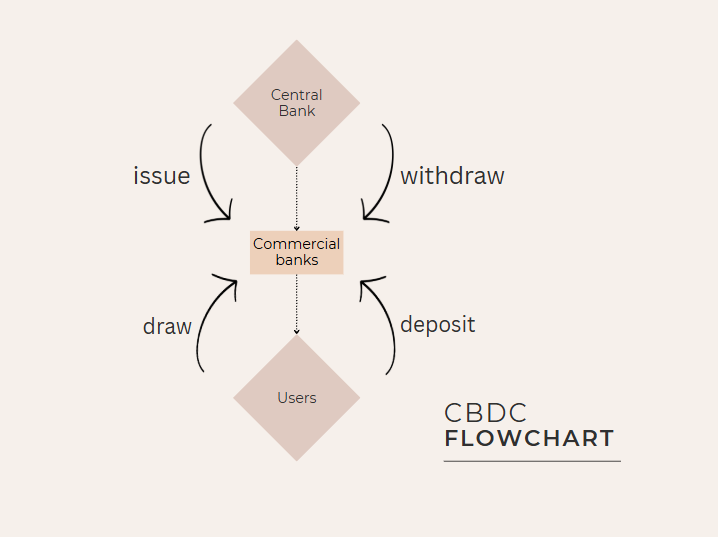
\includegraphics[width=0.8\linewidth]{image.png}
    \caption{Flow chart of CBDC architecture}
    \label{fig:enter-label}
\end{figure}
\begin{figure}
    \centering
    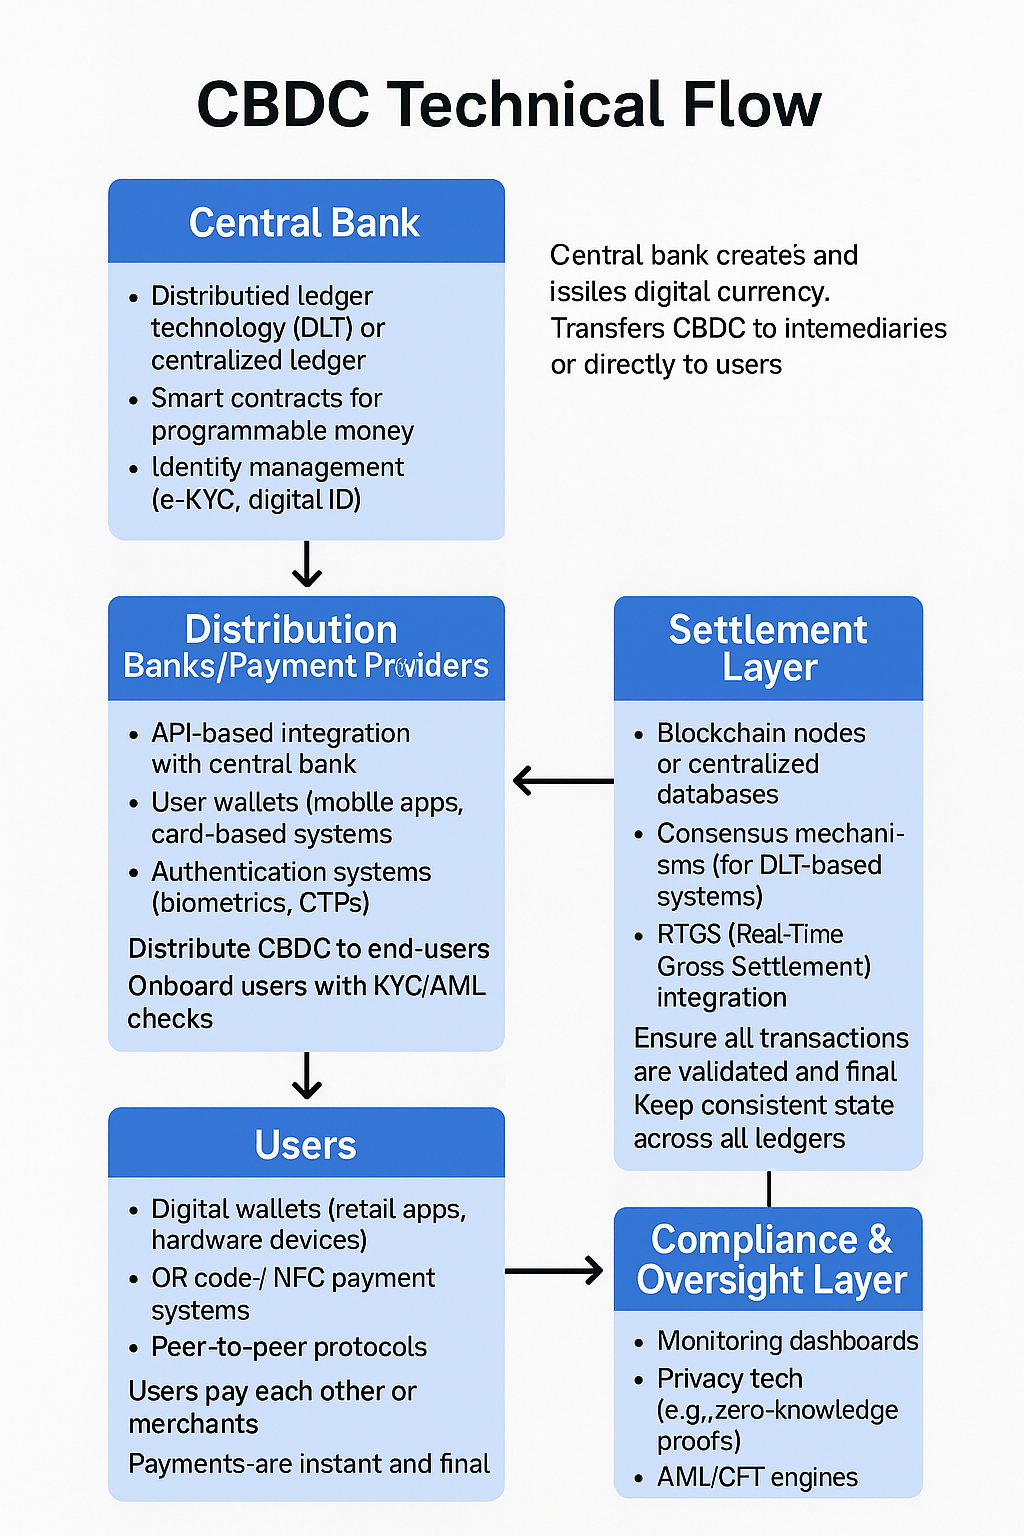
\includegraphics[width=0.8\linewidth]{image2.png}
    \caption{Proposed Architecture of CBDC for India}
    \label{fig:cbdc_architecture}
\end{figure}

\section{Ledger System}

The proposed CBDC architecture adopts a hybrid ledger model that brings together the strengths of both decentralized and centralized systems. At its core is a \textbf{permissioned Distributed Ledger Technology (DLT)}, designed to ensure that every transaction is secure, transparent, and efficiently recorded.

\begin{itemize}
    \item \textbf{Immutable Records:} Each transaction is cryptographically secured and permanently stored, ensuring data integrity.
    \item \textbf{Audit Trails:} The ledger maintains a complete and tamper-proof history of all transactions, which supports regulatory compliance and helps in detecting and preventing fraud.
    \item \textbf{High Scalability:} Optimized to handle millions of retail transactions in real-time, the system ensures smooth operation even under heavy load.
\end{itemize}

Alongside the DLT, the system also integrates a \textbf{centralized ledger} maintained by the Reserve Bank of India. This component plays a crucial role in managing monetary and regulatory functions efficiently.

\begin{itemize}
    \item \textbf{Central Oversight:} The RBI retains full authority over the issuance, distribution, and retirement of digital currency, ensuring policy control.
    \item \textbf{Policy Implementation:} Features like programmable money and interest-bearing CBDC can be implemented more seamlessly through centralized control.
    \item \textbf{Efficient Settlements:} High-value wholesale transactions can be settled quickly with reduced latency using centralized infrastructure.
\end{itemize}

This hybrid model strikes a balance between transparency and control—leveraging the innovation of distributed systems while preserving the central bank's ability to steer and supervise the financial ecosystem effectively.


\section{Token-based vs Account-based Models}

Given the diverse financial needs and digital maturity levels across India, the proposed CBDC model is designed to support both \textbf{token-based} and \textbf{account-based} approaches. This dual-model structure ensures flexibility, inclusivity, and alignment with varying use cases across the population.

\textbf{Token-based CBDC} operates much like physical cash in digital form. It is particularly well-suited for low-value transactions where privacy and ease of use are critical. Since ownership is validated through possession rather than identity, it allows for anonymous transactions, making it ideal for:

\begin{itemize}
    \item Peer-to-peer transfers in rural or underbanked areas.
    \item Offline payments where network access may be limited or unavailable.
    \item Small retail purchases where minimal friction and quick settlement are desired.
\end{itemize}

\textbf{Account-based CBDC}, on the other hand, functions similarly to a bank account. It requires identity verification and is directly linked to the user’s digital identity. This model is better suited for:

\begin{itemize}
    \item High-value or regulated transactions requiring KYC and AML compliance.
    \item Institutional and business payments where audit trails and accountability are necessary.
    \item Scenarios where programmable features or policy-driven restrictions (e.g., spending limits, taxation) are applied.
\end{itemize}

By integrating both models, the system accommodates a broad spectrum of users—from individuals seeking cash-like privacy to businesses and institutions requiring secure, regulated digital payments. This approach ensures that India's CBDC infrastructure remains inclusive, adaptable, and responsive to the evolving needs of its diverse economy.

\section{Stakeholders}

The success of the proposed CBDC ecosystem depends on seamless coordination among a range of stakeholders, each with a distinct and vital role. Together, they form an interconnected network that supports issuance, distribution, access, and everyday usage of the digital currency.

\begin{itemize}
    \item \textbf{Reserve Bank of India (RBI):}  
    As the sole issuer and regulator, the RBI oversees the creation, circulation, and overall governance of the CBDC. It ensures monetary policy alignment, sets operational guidelines, and maintains the integrity of the system.

    \item \textbf{Commercial Banks:}  
    Banks act as intermediaries between the RBI and end-users. They handle user onboarding through Know Your Customer (KYC) procedures, manage wallets and accounts, and facilitate the secure distribution of CBDC to individuals and businesses.

    \item \textbf{Payment Service Providers (PSPs):}  
    Fintech companies and digital wallet providers play a key role in delivering user-friendly platforms and mobile applications. Their focus is on enhancing user experience, enabling seamless retail payments, and ensuring broad accessibility—both online and offline.

    \item \textbf{Citizens and End Users:}  
    From tech-savvy urban professionals to rural individuals with limited digital exposure, citizens are at the heart of the CBDC ecosystem. Whether it's paying for groceries, sending money to family, or receiving government subsidies, the CBDC is designed to be intuitive and accessible for all.
\end{itemize}

By fostering collaboration across these stakeholders, the CBDC ecosystem ensures trust, efficiency, and inclusiveness—creating a foundation for a modern, digital economy that serves the entire population.

\section{Interoperability}

To ensure seamless integration with India’s current payment infrastructure, the CBDC is designed to work with:

\begin{itemize}
    \item \textbf{UPI, NEFT, RTGS:} For instant or scheduled transfers.
    \item \textbf{Wallets and POS:} Allowing both merchants and consumers to adopt CBDC without disruption.
\end{itemize}

\begin{figure}
    \centering
    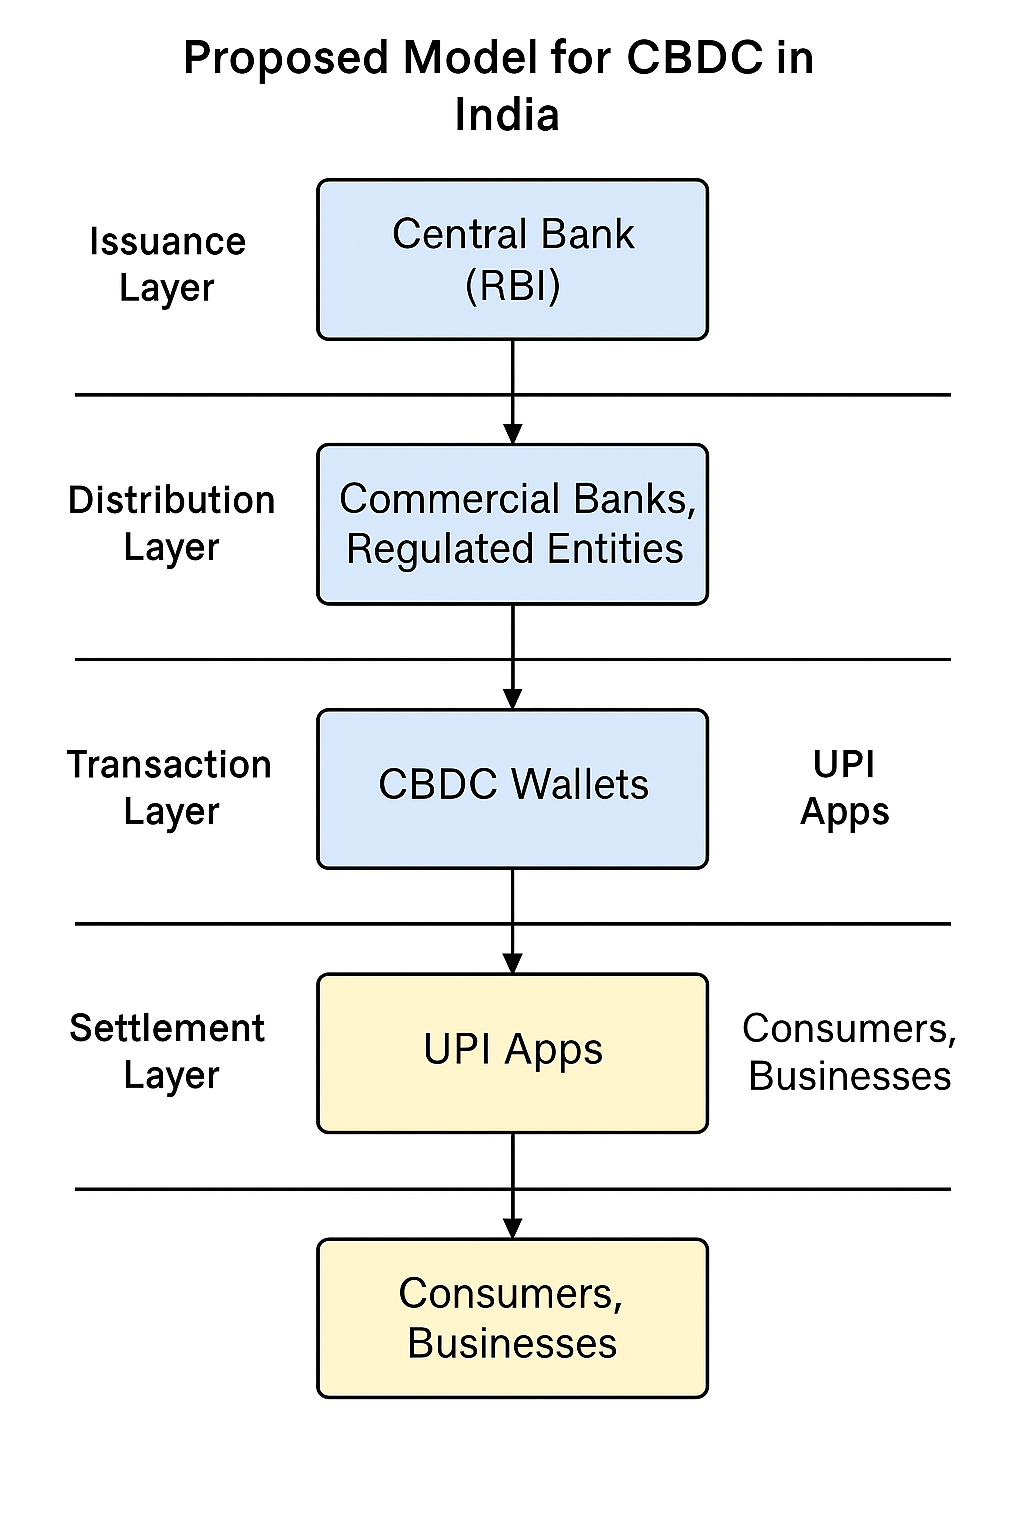
\includegraphics[width=0.75\linewidth]{image3.png}
    \caption{Flow chart of the model}
    \label{fig:enter-label}
\end{figure}
\section{Offline Capability}

One of the major strengths of this model is its ability to function even in areas with poor connectivity. Offline CBDC access can be enabled via:

\begin{itemize}
    \item \textbf{NFC-enabled smart cards}
    \item \textbf{QR code-based wallet apps}
    \item \textbf{Bluetooth-based peer-to-peer payments}
\end{itemize}

\section{Privacy and Security}

Security and privacy are built into the system through a \textbf{tiered KYC framework}, offering different levels of anonymity based on transaction size and use-case.

\begin{itemize}
    \item \textbf{Low-value transactions:} Allow pseudonymous access, preserving user privacy.
    \item \textbf{High-value payments:} Require full KYC and digital audit trails.
    \item \textbf{Advanced privacy tools:} Such as Zero-Knowledge Proofs (ZKPs) can be incorporated for enhanced confidentiality.
\end{itemize}

\section{Smart Contract Support}

To future-proof the CBDC system, the architecture supports smart contracts, enabling programmable financial tools such as:

\begin{itemize}
    \item \textbf{Time-bound payments:} Automatically revoke unclaimed subsidies after a deadline.
    \item \textbf{Conditional transfers:} For government benefits tied to specific uses.
    \item \textbf{Escrow mechanisms:} For safer e-commerce and service transactions.
\end{itemize}
\vspace{-5mm}
\section{Summary}
In summary, the proposed hybrid CBDC model is thoughtfully designed to address the diverse and evolving needs of India's economy and its people. It emphasizes \textbf{inclusivity}, ensuring that individuals across all regions---urban or rural, digitally connected or offline---can access and use digital currency with ease. The model is \textbf{scalable}, capable of handling the high volume and complexity of transactions in one of the world's most populous nations, while remaining \textbf{secure} through advanced technologies such as permissioned distributed ledger systems and tiered identity verification.
By integrating the strengths of India’s existing financial infrastructure---such as UPI, mobile wallets, and traditional banking---with modern digital innovations like offline payments, tokenization, and smart contracts, this CBDC model enables a \textbf{smooth and practical transition} toward a digital monetary system. Importantly, it reinforces public \textbf{trust} by maintaining central bank oversight, ensures \textbf{financial accessibility} even in underserved communities, and protects \textbf{monetary sovereignty} by offering a public alternative to private cryptocurrencies.
Ultimately, this hybrid architecture lays the foundation for a \textbf{resilient and future-ready digital economy}, where public digital money coexists and interoperates seamlessly with current systems, empowering citizens, businesses, and the broader financial ecosystem.\\\\\\\\\\
\pagebreak
\cleardoublepage
\clearpage
%%%%%%%%%%%%%%%%%%%%%%%%%%%%%%%%%%%%%%%%%%%%%%%%%%%%%%%%%%%%%%%%%%%%%%%%%%%%
%% Chapter 5
%%Indian Institute of Information Technology Kalyani
%% All rights are reserved.
%%%%%%%%%%%%%%%%%%%%%%%%%%%%%%%%%%%%%%%%%%%%%%%%%%%%%%%%%%%%%%%%%%%%%%%%%%%%

\chapter{Technical Implementation}
\label{chp5}

Designing a Central Bank Digital Currency (CBDC) system goes beyond simply digitizing cash. It requires creating a secure, efficient, scalable, and inclusive ecosystem capable of serving a diverse population like India's. This chapter outlines the technical blueprint for how such a system could be developed and implemented. While this work does not present a fully functional prototype, it provides a detailed analysis of the tools, architecture, and technologies essential to realizing an operational CBDC framework for India.

\section{Tools and Frameworks Considered}
Developing a CBDC involves selecting technologies that can ensure security, scalability, interoperability, and accessibility. Based on the unique demands of implementing a national-level digital currency, the following tools and frameworks have been evaluated:

\subsection*{Distributed Ledger Technology (DLT)}
DLT ensures secure and tamper-resistant transaction records. The following platforms are considered suitable:
\begin{itemize}
    \item \textbf{Hyperledger Fabric:} Permissioned, enterprise-grade blockchain ideal for regulated environments.
    \item \textbf{Ethereum:} A public blockchain platform with broad adoption and smart contract support.
    \item \textbf{Corda:} Tailored for financial institutions, supporting privacy and transaction control.
\end{itemize}

\subsection*{Simulation Tools}
Simulating system behavior before deployment helps evaluate robustness under various conditions. Tools include:
\begin{itemize}
    \item \textbf{MATLAB:} Useful for modeling control systems and network behavior.
    \item \textbf{AnyLogic:} Allows detailed simulation of transaction flows, failures, and network loads.
\end{itemize}

\subsection*{Wallet SDKs and APIs}
User interaction relies heavily on mobile interfaces. Development tools include:
\begin{itemize}
    \item \textbf{UPI APIs:} For secure and instantaneous fund transfers.
    \item \textbf{Flutter and React Native:} Enable cross-platform mobile wallet development.
\end{itemize}

\section{Architecture Overview}
The CBDC architecture is designed as a hybrid model, combining centralized governance with decentralized access. Key components include:
\begin{itemize}
    \item \textbf{Central Bank (RBI):} Responsible for issuance, policy control, and system oversight.
    \item \textbf{Commercial Banks and PSPs:} Serve as intermediaries, distributing CBDC and managing user accounts.
    \item \textbf{End Users:} Citizens, merchants, and government bodies interact with the CBDC via wallets.
\end{itemize}

This layered approach retains centralized security and trust while distributing operational workload across financial intermediaries.

\begin{figure}[H]
\centering
% \fbox{\includegraphics[width=0.8\textwidth]{Figure/chp5/architecture-diagram.png}}
\caption{Proposed Architecture of the CBDC System}
\label{fig:chp5-architecture}
\end{figure}

\section{Data Flow and Process}
A standard transaction in the CBDC system follows these steps:
\begin{enumerate}
    \item \textbf{User Authentication:} Verified through Aadhaar-based eKYC, biometric data, or device-level checks.
    \item \textbf{Transaction Initiation:} Users scan QR codes or enter recipient details to initiate payments.
    \item \textbf{Ledger Update:} Transactions are recorded on the distributed ledger, ensuring transparency and immutability.
    \item \textbf{Transaction Confirmation:} Both sender and receiver receive real-time confirmation of the transfer.
\begin{figure}
    \centering
    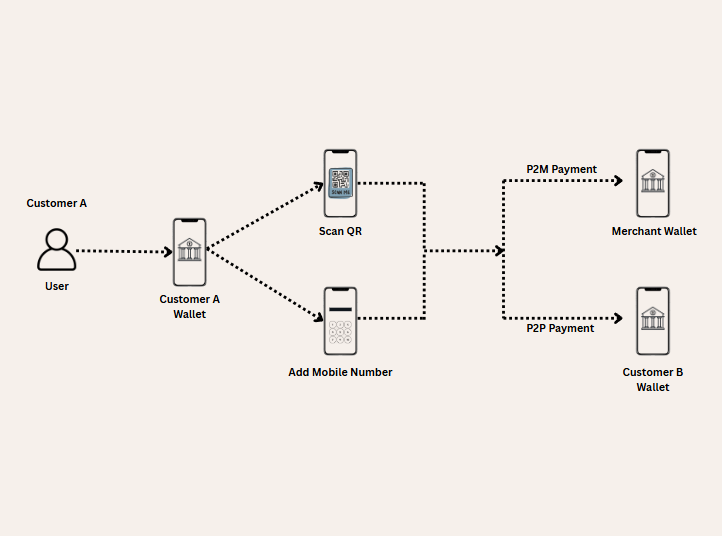
\includegraphics[width=0.9\linewidth]{chp5img1.png}
    \caption{Transaction by User Flowchart}
    \label{fig:enter-label}
\end{figure}
\end{enumerate}
This end-to-end flow ensures security, speed, and integrity in every transaction.

\section{Use Case Scenarios}
CBDC has broad applicability. Key scenarios include:
\begin{itemize}
    \item \textbf{Retail Transactions:} Instant payments in physical and online stores.
    \item \textbf{Peer-to-Peer Transfers:} Seamless fund movement between individuals.
    \item \textbf{Government Payments:} Direct Benefit Transfers (DBT) and subsidies without intermediaries.
    \item \textbf{Offline Usage:} Payments in no-network zones via NFC cards or QR-enabled devices.
\end{itemize}

\section{Security Considerations}
Given its financial nature, the CBDC system integrates multiple security layers:
\begin{itemize}
    \item \textbf{Double-Spending Prevention:} Unique token IDs ensure each unit is spent only once.
    \item \textbf{Cryptographic Security:} Public-private keys secure all wallet operations.
    \item \textbf{Counterfeit Protection:} Digital watermarking verifies currency authenticity.
    \item \textbf{Infrastructure Resilience:} Load balancing, backups, and failover systems ensure availability.
\end{itemize}

\section{Conclusion}
Implementing a CBDC at a national scale is an ambitious but transformative goal. It requires the fusion of advanced technologies with the stability and trust of traditional finance. The proposed hybrid system architecture, powered by a robust technology stack, enables secure, efficient, and inclusive access to digital money.

Although this chapter presents a conceptual design rather than a functional system, it offers a practical foundation upon which India can build its CBDC. Future steps involve prototyping, pilot testing, and policy alignment to transition from theoretical models to real-world applications, ensuring that digital currency becomes a reality for every citizen---regardless of geography or connectivity.

\cleardoublepage
%%%%%%%%%%%%%%%%%%%%%%%%%%%%%%%%%%%%%%%%%%%%%%%%%%%%%%%%%%%%%%%%%%%%%%%%%%%%
%% Chapter 6
%%Indian Institute of Information Technology Kalyani
%% All rights are reserved.
%%%%%%%%%%%%%%%%%%%%%%%%%%%%%%%%%%%%%%%%%%%%%%%%%%%%%%%%%%%%%%%%%%%%%%%%%%%%
%
    \chapter{Benefits and Challenges}
\label{chp6}

As the world steadily transitions towards a more digital economy, Central Bank Digital Currencies (CBDCs) have emerged as a major innovation with the potential to reshape how we interact with money. These digital versions of fiat currency, issued and regulated by central banks, offer numerous advantages over traditional forms of currency, but they also come with a unique set of challenges that need careful consideration.

This chapter explores the tangible benefits of CBDCs, as well as the obstacles that policymakers, governments, and central banks must navigate for successful implementation.

\section{Benefits of CBDC}
CBDCs are not merely a digital alternative to cash; they represent a new foundation for a more efficient, inclusive, and innovative financial ecosystem. Here are some of the key benefits:

\subsection{Reduced Transaction Costs}
One of the most immediate benefits of CBDCs is the potential to lower the cost of everyday transactions. In traditional systems, payments often pass through several intermediaries—such as commercial banks, payment gateways, or clearinghouses—each adding their own processing fees.

CBDCs allow for direct peer-to-peer payments, reducing or even eliminating these intermediary costs. This makes transactions faster, cheaper, and more accessible—especially for micro-payments or remittances. For businesses, particularly small and medium enterprises (SMEs), this could significantly reduce operational overheads and improve cash flow efficiency.

\subsection{Enhanced Monetary Control}
From a central bank’s perspective, CBDCs provide greater precision in implementing monetary policy. Currently, much of the money circulating in the economy is in commercial bank accounts, where central banks have only indirect influence through tools like interest rates or reserve requirements.

With CBDCs, central banks could directly influence money supply and liquidity in real-time. This opens up opportunities for:

\begin{itemize}
    \item More effective control over inflation and deflation
    \item Real-time interest rate adjustments
    \item Automatic fiscal interventions during crises (e.g., direct transfers during pandemics)
\end{itemize}

CBDCs could be a powerful tool in maintaining macroeconomic stability and responding quickly to economic shocks.

\subsection{Financial Inclusion}
Perhaps one of the most socially impactful benefits of CBDCs is their ability to reach the unbanked and underbanked populations. In countries like India, where millions still lack access to traditional banking services, CBDCs could bridge the gap between formal financial institutions and those excluded from them.

With nothing more than a basic smartphone or a digital ID, individuals could:

\begin{itemize}
    \item Receive salaries, pensions, or government benefits directly
    \item Make secure and instant payments
    \item Save money without needing a traditional bank account
\end{itemize}

For rural areas, tribal communities, or migrant workers, CBDCs could empower people to participate more actively in the economy.

\subsection{Programmable Money and Innovation Potential}
CBDCs introduce the revolutionary concept of programmable money—digital currency that can be coded to behave in specific ways.

Imagine welfare payments that can only be used for essentials like groceries or healthcare, or business subsidies that expire if not used within a fiscal year. Programmable features can be integrated to improve transparency, reduce misuse, and automate compliance.

Furthermore, this lays the foundation for:

\begin{itemize}
    \item Smart contracts for business automation
    \item Automatic tax deductions at point-of-sale
    \item Conditional payments (e.g., escrow releases only when service is completed)
\end{itemize}

This level of flexibility is impossible with physical cash or even traditional digital banking systems.

\section{Challenges of CBDC Implementation}
While the potential benefits are impressive, implementing a CBDC system is not without its complexities. Governments and financial institutions will need to navigate multiple technical, social, and economic challenges.

\subsection{Balancing Privacy and Regulation}
One of the thorniest issues in CBDC deployment is finding the right balance between user privacy and regulatory oversight.

On the one hand, people expect their transactions to remain private—especially for small, everyday purchases. On the other hand, governments and regulators need transparency to combat money laundering, tax evasion, and terrorism financing.

Too much surveillance could lead to public distrust and resistance. Too much privacy could compromise national security. The challenge lies in designing a system that respects individual freedom while complying with legal and ethical standards.

\subsection{Technological Literacy and Accessibility}
Digital systems assume a certain level of technological comfort. However, many users—especially the elderly, rural populations, and those with limited education—might struggle to adopt CBDCs.

This makes digital literacy and public education essential. Governments and central banks must:

\begin{itemize}
    \item Conduct awareness campaigns
    \item Provide hands-on training
    \item Ensure multilingual and intuitive app interfaces
    \item Offer alternatives for people without smartphones or stable internet
\end{itemize}

Inclusion cannot be achieved if the system is too complex or inaccessible.

\subsection{Infrastructure Development and Cost}
Setting up a CBDC system requires robust and secure infrastructure—including national-level servers, encrypted databases, mobile apps, payment gateways, and offline access solutions.

Developing and maintaining this digital backbone involves significant upfront investment. In developing economies, this may stretch existing financial and technical resources. Additionally, continuous updates and cybersecurity upgrades will be required to stay ahead of evolving threats.

The trade-off between cost and benefit must be evaluated carefully, especially when scaling the system to millions of users.

\subsection{Cybersecurity Risks and Threats}
As CBDCs go digital, they become vulnerable to the same risks that plague any online system—hacking, data breaches, system outages, or denial-of-service attacks.

If a CBDC system were compromised, it could shake public confidence, disrupt economies, and lead to massive financial loss. Thus, cybersecurity must be baked into the design, not added later as a patch.

This includes:

\begin{itemize}
    \item Multi-layered encryption
    \item Real-time threat monitoring
    \item Redundant backup systems
    \item Biometric or multi-factor authentication for users
\end{itemize}

A single breach could have national consequences, so resilience and trust are non-negotiable.

\subsection{Disruption to Traditional Financial Systems}
CBDCs could pose a disruptive threat to existing banks and payment processors. If citizens can hold money directly with the central bank, commercial banks might see reduced deposits, affecting their ability to lend and operate profitably.

Similarly, private payment apps may face competition from government-run CBDC wallets with lower transaction costs.

To avoid destabilizing the financial ecosystem, policymakers will need to design a two-tier system, where commercial banks and fintechs continue to play an active role, possibly as CBDC distributors or service providers.

\subsection{Cross-Border Transaction and Interoperability Issues}
CBDCs will truly unlock their potential when they work across borders, enabling fast, cheap, and secure international remittances or trade settlements.

However, this is easier said than done. Each country has different:

\begin{itemize}
    \item Technical standards
    \item Privacy laws
    \item Monetary policies
    \item Geopolitical concerns
\end{itemize}

Building interoperability protocols, creating bilateral/multilateral agreements, and aligning regulatory frameworks will be a long but necessary journey to global adoption.

\section{Conclusion}
CBDCs are not just a technological upgrade—they are a paradigm shift in how money is issued, managed, and used. The promise of lower costs, greater inclusion, programmable transactions, and improved monetary control makes CBDCs an attractive proposition for modern economies.

However, for this vision to succeed, the challenges must be acknowledged and addressed head-on. Privacy concerns, technical education, infrastructure readiness, and cybersecurity are not minor hurdles—they are core components of any CBDC initiative.

If done thoughtfully, CBDCs can democratize finance, empower marginalized communities, and build a more transparent, resilient, and innovative financial system for future generations. But the road ahead requires collaboration between central banks, governments, technologists, and citizens alike.


\cleardoublepage
%%%%%%%%%%%%%%%%%%%%%%%%%%%%%%%%%%%%%%%%%%%%%%%%%%%%%%%%%%%%%%%%%%%%%%%%%%%%
%% Chapter 7
%%Indian Institute of Information Technology Kalyani
%% All rights are reserved.
%%%%%%%%%%%%%%%%%%%%%%%%%%%%%%%%%%%%%%%%%%%%%%%%%%%%%%%%%%%%%%%%%%%%%%%%%%%%
%
\chapter{Future Scope}
\label{chp7}

Central Bank Digital Currencies (CBDCs) represent one of the most significant developments in the modern financial era. As we stand at the threshold of this digital transformation, it’s clear that the journey is only just beginning. While initial experiments and pilot projects are paving the way, the full potential of CBDCs is yet to be realized. This chapter explores the promising directions that CBDC research and implementation could take in the years to come.

\section{Integration with International CBDCs}

In an increasingly globalized world, money must move across borders as effortlessly as it moves within them. One of the most exciting frontiers for CBDCs is their potential to integrate with other nations’ digital currencies, enabling frictionless international payments.

As countries like China, Sweden, and the European Union develop their own digital currencies, there is a growing need to establish interoperable systems that can support seamless cross-border transactions. A CBDC that can "speak the language" of another country's digital currency could reduce foreign exchange costs, accelerate international trade settlements, and lessen dependency on intermediaries such as correspondent banks or SWIFT.

For instance, if India's digital rupee could directly interact with China's e-CNY or the European Central Bank's digital euro, international trade could become faster, cheaper, and more secure. Achieving this vision will require global collaboration on technical standards, regulatory harmonization, and diplomatic cooperation.

\section{Leveraging AI for Fraud Detection and Risk Mitigation}

As digital transactions increase, so does the sophistication of financial fraud. Traditional fraud detection systems are often reactive and rule-based, struggling to keep pace with evolving threats. In contrast, Artificial Intelligence (AI) has the potential to offer proactive and adaptive security solutions.

Machine learning algorithms can analyze vast amounts of CBDC transaction data in real time, identifying anomalies that suggest fraudulent activity, money laundering, or other financial crimes. Unlike static rules, AI systems can continuously learn from new data, improving their accuracy over time.

Moreover, AI-driven risk scoring models could help central banks assess systemic risks in the digital economy, enabling more responsive monetary policy. These intelligent systems could serve as an early warning mechanism, safeguarding both users and institutions from large-scale disruptions.

\section{Enhancing Offline Functionality}

While CBDCs are fundamentally digital, their usefulness should not be limited by internet connectivity. In a country like India, where millions still live in areas with intermittent or no internet access, enabling offline transactions is not just a convenience—it’s a necessity.

Future CBDC systems should support offline payments using technologies like Bluetooth, NFC (Near-Field Communication), or secure hardware wallets. This would allow users in rural or underserved regions to send and receive money without a network connection, fostering financial inclusion.

Offline capabilities could also be vital in disaster scenarios—natural calamities, internet outages, or cyberattacks—where digital payments might otherwise become inaccessible. Creating a resilient, offline-compatible CBDC ecosystem will be crucial for nationwide adoption and trust.
\clearpage
\section{Interoperability with DeFi and Crypto Ecosystems}

As decentralized finance (DeFi) continues to grow, a major question emerges: can CBDCs interact meaningfully with these decentralized systems?

In the future, bridges between CBDCs and crypto platforms could allow for the exchange of central bank-issued currency with digital assets like Bitcoin, Ethereum, or stablecoins. This interoperability would offer users more flexibility, letting them move funds across ecosystems while enjoying the security of CBDCs and the innovation of DeFi.

For example, a user could convert digital rupees into a DeFi token to earn interest through lending protocols, or use smart contracts to automate payments—all while staying anchored to a sovereign-backed currency. Such integrations would require new technical protocols and regulatory clarity, but they hold the potential to reshape the boundaries between centralized and decentralized finance.

\section{Expanding Use Cases for CBDCs}

CBDCs can do far more than just replace cash or facilitate retail payments. With programmable capabilities and integration into digital infrastructure, their use cases could expand across various sectors:

\subsection{Programmable Money for Government Initiatives}

One of the most powerful features of CBDCs is programmability—the ability to embed conditions into how the money is used. Governments could leverage this to deliver welfare payments, subsidies, or emergency relief directly to citizens’ digital wallets. For instance, stimulus funds could be programmed to expire after a certain period, encouraging immediate spending to stimulate the economy. Alternatively, funds could be restricted to specific categories like food, healthcare, or education, ensuring targeted support.

\subsection{Corporate Applications and Treasury Management}

Corporations could benefit from CBDCs by using them for payroll, supplier payments, or internal fund transfers. This would streamline processes, reduce transaction costs, and enable automated financial operations through smart contracts.

Additionally, programmable CBDCs could simplify tax reporting, compliance, and auditing for businesses by maintaining transparent and immutable transaction records.

\subsection{Digital Identity Integration}

Another important future direction is the integration of digital identity frameworks with CBDCs. A secure, government-verified digital identity linked to CBDC wallets could improve KYC compliance, reduce fraud, and simplify onboarding for financial services.

This would be especially transformative in regions where many people lack formal identification or access to banking, opening the door to new financial opportunities through a secure and user-friendly digital platform.

\subsection{Decentralized and Centralized Exchanges}

As the digital currency ecosystem grows, the need for robust exchange platforms will also increase. Future CBDC systems could support both centralized exchanges (managed by governments or banks) and decentralized ones (run on blockchain protocols), giving users more options to manage and convert their digital assets. These platforms could facilitate CBDC-to-crypto swaps, enable tokenized assets trading, or support digital securities—all within a legally compliant and secure environment.

\section{Conclusion}

The journey of CBDCs is still in its early stages, but the path ahead is rich with potential. From enabling inclusive offline payments to fostering international cooperation and unlocking programmable money, CBDCs are poised to redefine how we interact with money itself.

As technology, regulation, and user expectations evolve, so too must CBDC frameworks. Their success will depend on a careful balance of innovation, security, scalability, and human-centered design. It’s not just about digitizing currency; it’s about reimagining the future of finance.

Ongoing research and experimentation will play a critical role in navigating this transition. As central banks, policymakers, technologists, and communities continue to collaborate, CBDCs could become a cornerstone of a more resilient, transparent, and equitable financial world.

\cleardoublepage
%%%%%%%%%%%%%%%%%%%%%%%%%%%%%%%%%%%%%%%%%%%%%%%%%%%%%%%%%%%%%%%%%%%%%%%%%%%%
%% Chapter 8
%%Indian Institute of Information Technology Kalyani
%% All rights are reserved.
%%%%%%%%%%%%%%%%%%%%%%%%%%%%%%%%%%%%%%%%%%%%%%%%%%%%%%%%%%%%%%%%%%%%%%%%%%%%
%
\chapter{Conclusion}
\label{chp8}

This thesis set out to explore the rapidly evolving world of Central Bank Digital Currencies (CBDCs) and their possible role in India’s financial system. As we come to the end of this study, it’s important to reflect on the key takeaways, evaluate the feasibility of the model we proposed for India, and think about what CBDCs might mean for the future of digital finance.

\section{Summary of Findings}

Throughout this research, several important points emerged:

\begin{itemize}
    \item Around the world, people are moving more and more towards digital payments, using cash less frequently. This shift is encouraging central banks to rethink how money is issued and controlled.
    \item CBDCs offer central banks a way to keep control over the currency while addressing problems like financial exclusion, lack of transparency, and inefficiency.
    \item The model proposed here takes into account India’s unique financial situation. It aims to handle challenges such as supporting a huge population, enabling secure offline transactions, and protecting user privacy.
    \item For CBDCs to be widely accepted, they need to work smoothly with existing payment systems like UPI and e-wallets.
    \item CBDCs could bring many benefits — lower transaction costs, faster payments, broader access to banking — but they also come with challenges such as cybersecurity risks and the need for strong regulations.
    \item Looking ahead, CBDCs might connect with international payment networks, integrate with emerging finance technologies, and use AI to fight fraud.
\end{itemize}

\section{Feasibility of the Proposed Model}

The model presented in this thesis is practical and fits well with India’s growing digital economy. It is designed to be flexible, secure, and able to work both in cities and remote areas. Still, its success depends on several key factors:

\begin{itemize}
    \item \textbf{Supportive Policies:} Clear laws and cooperation between institutions are essential. Current legal frameworks will need updates to cover digital currencies.
    \item \textbf{Strong Technology:} The infrastructure must be safe, reliable, and scalable, including ways to handle transactions offline in areas without internet.
    \item \textbf{User Acceptance:} People and organizations need to understand and trust the system. Awareness campaigns and digital literacy programs will be important.
    \item \textbf{Privacy and Security:} Trust depends on protecting users’ data through strong encryption and secure identity verification.
\end{itemize}

\section{Final Thoughts}

CBDCs are not just another digital innovation — they have the potential to change how money is issued, circulated, and controlled in the digital age. For India, with its diverse population and robust digital systems like Aadhaar and UPI, a well-designed CBDC could be a game-changer.

But there are challenges to overcome. Legal frameworks, technology, and social acceptance all need to develop together. Issues like data privacy and digital literacy require attention, and collaboration between policymakers, tech experts, banks, and the public will be key.

\section{Suggestions for Future Research}

While this thesis lays some groundwork, there’s still much to explore:

\begin{itemize}
    \item How can CBDCs work smoothly across countries? Research into international standards and cooperation is needed.
    \item What are the pros and cons of using blockchain versus traditional databases for CBDCs?
    \item How do people really feel about digital currencies? Understanding user trust and privacy concerns is important.
    \item How well do CBDCs actually help people who don’t have easy access to banks? Measuring real-world impact is crucial.
\end{itemize}

The journey to bring CBDCs to India has only just begun. Ongoing research, pilot projects, and open conversations will be vital to build a digital currency system that is not only technologically strong but also inclusive and trusted by all.

\cleardoublepage
%%\begin{flushleft}
%{\Large \textsc{\textbf{Publications}}}
%\end{flushleft}
\chapter*{Publications}
%\rule{\textwidth}{0.4pt}\par % Thick horizontal line
This thesis is based on some of the following publications of the author.\\


%\addcontentsline{toc}{chapter}{Publications}
%\printglossary[style=long]
\bibliographystyle{ieeetr}
\cleardoublepage
\bibliography{Reference/Bibliography.bib}
\end{document}